\section{Maschine Learning}

Der Fokus dieser Arbeit ist die Ermittlung von Design von Quellcode durch die Anwendung von Maschine Learning.
Dieser Teil der Arbeit ist für die Erläuterung von verwendeten Metriken, angewandten Techniken und ausgewählter Klassifizierer gewidmet.

% TODO: \subsection{Terminologie} falls notwendig
\subsection{Metriken für Evaluierung von Modellen}

Um die Leistung eines Klassifizierers zu ermitteln, bedarf es einer Menge an Metriken, womit beurteilt werden, ob der Klassifizierer wie erwartet performt.
In Kontext dieser Aussage wird in der Domäne des Maschine Learnings bekannte Metriken aus dem Bereich der Statistik angewendet.
In diesem Abschnitt wird eine Auswahl von solchen Metriken erläutert, die in der Literaturrecherche als auch in den Sektionen der Methodik und Implementierung erwähnt werden.
Für die Ermittelung der Metriken werden folgende Größen definiert:

\begin{description}
    \item TP (True Positive): Anzahl echt positiver Klassifizierungen
    \item TN (True Negative): Anzahl echt negativer Klassifizierungen
    \item FP (False Postive): Anzahl falsch positiv Klassifizierungen
    \item FN (False Negative): Anzahl falsch negativ Klassifizierungen
\end{description}

Anhand dieser Größen werden folgende Metriken definiert:

\begin{description}
    \item \textit{Accuracy (Genauigkeit)}: Dieser Wert gibt an, wie das Verhältnis zwischen den klassifizierten Beobachtungen zur Gesamtzahl der Beobachtungen ist.
    \\
    \\
    $Accuracy = \frac{\text{Anzahl der korrekten Vorhersagen}}{\text{Gesamtzahl der Vorhersagen}} = \frac{TP+TN}{TP+TN+FP+FN}$

    \item \textit{Precision (Präzision)}: Dieser Wert gibt das Verhältnis an, wie die korrekt positiv klassifizierten Beobachtungen zur Gesamtzahl der als positiv klassifizierten Beobachtungen stehen.
    \\
    \\
    $Precision = \frac{TP}{TP+FP}$

    \item \textit{Recall (Sensitivität)}: : Dies ist das Verhältnis der positiv klassifizierten Beobachtungen zur Gesamtzahl der tatsächlichen positiven Beobachtungen.
    \\
    \\
    $Recall = \frac{TP}{TP+FN}$
    
    \item \textit{ F1-Score}: Der F1-Score ist das harmonische Mittel von Präzision und Recall und gibt ein besseres Maß für die unbalancierten Klassen als die Genauigkeit allein.
    \\
    \\
    $\textit{\text{F1-Score}} = 2 * \frac{Precision * Recall}{Precision + Recall} = \frac{2*TP}{2*TP + FP + FN}$
\end{description}

\pagebreak

\subsection{Validierung und Optimierung von Modellen}

Neben dem Zusammentragen von relevanten Datenpunkte für die Erhebung eines geeigneten Datensatzes ist das Validierung und Optimierung des Maschine Learning Modells eines der relevanten Schritte im gesamten Prozess, 
um damit das Modell dessen Aufgabe möglichst zufriedenstellend erfüllen kann. 
In diesem Teil der Arbeit werden Techniken bzw. Methoden erläutert, die in der Validierungs- oder Optimierungsphase angewendet werden können.


\subsubsection{Kreuzvalidierung von Modellen}
Nach dem Trainieren des Modells für einen Datensatz ist von Interesse, wie das Modell neue unbekannte Datenpunkte umgeht und diese Leistung anhand einer Metrik zu messen.
Dies stellt den Kernpunkt der Validierungsphase dar. Ein naiver Ansatz, die gleiche Menge an Datenpunkten zu verwenden, worauf das Modell in der Trainingsphase trainiert wurde.
Dabei ist jeder Datenpunkt des Datensatzes dem Modell bereits bekannt, wodurch es nicht auf wirklich unbekannte Datenpunkte validiert.
Eine Möglichkeit dem entgegenzukommen ist das Aufteilen des Datensatzes in Trainings- und Validationsdatensatz, wobei meist der Trainingsdatensatz die größere Menge an Datenpunkten zugesprochen wird.
Jedoch besteht hier der Nachteil, das in der Trainingsphase die Datenpunkte in dem Validationsdatensatz wegfallen.
Um diesen Nachteil zu negieren, kann die Technik der Cross Validation oder Kreuzvalidierung angewendet werden.

Hierbei wird zunächst eine natürliche Zahl \textit{n} bestimmt, die angibt, in wie viele gleich große Teile der Datensatz aufgeteilt wird.
Die Trainings- und Validierungsphase wird hierbei zu einem Schritt zusammengefasst und das Modell wird iterativ \textit{n}-Mal trainiert und anhand der vorgegebenen Metrik evaluiert.

\begin{figure}[h]
    \centering
    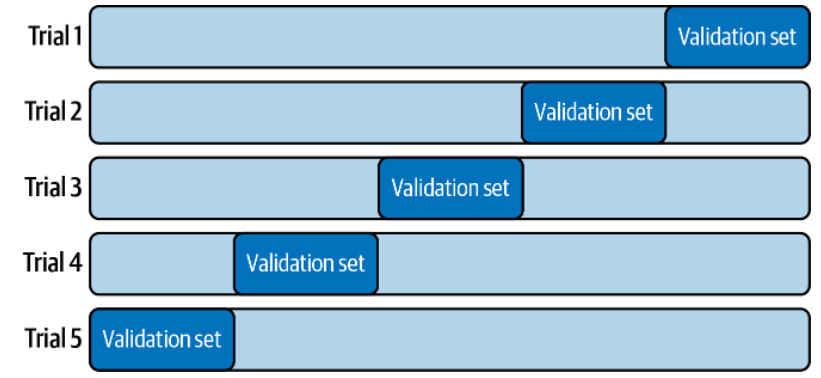
\includegraphics[scale=0.5]{figures/cross_validation}
    \caption{Kreuzvalidierung mit \textit{n} = 5}
    \label{fig:cross_validation}
\end{figure}
Wie aus Abbildung \ref{fig:cross_validation} zu entnehmen ist, wird in der \textit{i}-ten Iteration das $k-i$-te Sektion des Datensatzes für die Validierung und restlichen
für das Training des Modells verwendet. Das Resultat dieser Operation ist abhängig von Implementierung der Kreuzvalidierung die Iteration des Modells mit der besten Evaluation und eine Liste von Werten, die Leistung des Modells in der jeweiligen Iteration angibt.

\pagebreak

\subsubsection*{Optimieren von Modellen durch Hyperparameter-Tuning}
Maschine Learning Modelle können mithilfe von Parametern konfiguriert werden. Dabei wird zwischen zwei Arten von Parametern entschieden: Modellparameter und Hyperparameter.
Modellparameter werden während der Trainingsphase automatisiert direkt durch den Trainingsdatensatz bestimmt und sind nicht von Außen zu manipulieren. Dahingegen bestimmen Hyperparameter unter anderem wie sich das Modell während der Trainingsphase zu verhalten und beeinflussen
dessen Architektur. Jedes Modell definiert hierbei selbst, welche Hyperparameter verfügbar sind. Hyperparameter werden während der Instantiierung des Modells definiert. Die Ermittelung der bestmöglichen Kombinationen an Hyperparametern-Werten ist hilfreich, falls Leistung des Modells nicht den Erwartungen entspricht und das verwendete Datensatz nicht weiter argumentiert werden kann.
Um die Leistung des Modells zu evaluieren, wird wie in der Kreuzvalidierung eine Metrik bestimmt, die Leistung der jetzigen Iterationen zu beurteilen. Das Ziel der Hyperparameter-Optimierung besteht hier darin, eine Kombination an Hyperparametern-Werten zu bestimmen, wodurch die Metrik maximiert bzw. minimiert. 
Dies kann entweder manuell durchgeführt oder es werden Methoden eingesetzt, die dies automatisiert erledigen können. Im Folgendem wird eine Auswahl an automatisierten Strategien aufgelistet und erläutert:

\begin{description}
    \item Random Search/Grid Search: In diesen Methoden werden zunächst Wertebereiche für die jeweiligen Hyperparameter bestimmt. In der Regel wird hierbei eine Menge an diskreten Wertem bestimmt, die der jeweilige Hyperparameter annehmen kann. Jede Permutation der Hyperparameter-Konfiguration wird als eine Zelle in einem Gitter erfasst. 
    Jede besuchte Zelle dient dabei als Konfiguration für eine neue Instanz des Modells, welches im weiteren Verlauf durch Einsatz von Kreuzvalidierung trainiert und evaluiert wird. Das Ergebnis der Evaluation wird vermerkt.
    Bei Random Search wird zufällig bestimmt, welche Zellen besucht werden, während bei Grid Search alle Zellen besucht werden. Das Ergebnis ist die Konfiguration des Modells mit der besten Evaluierung.
    
    \item Bayessche Optimierung: Bei Grid bwz. Random Search wird jede Permuation der Hyperparameter-Werte eine Instanz des Modells traniert und evaluiert. Unter Umständen kann der Trainingsprozess je nach Modell und Datensatz rechenintensiv, wodurch es lange dauern, bis diese Methoden ein Resultat liefern.
    In solch einem Fall kann das Verfahren der Bayesschen Optimierung angewendet, um die Dauer der Evaluierung zu verkürzen. Im Kern wird das Maschine Learning Modell als Black Box Funktion interpretiert, welches als Eingabe eine Permuation an Hyperparameter-Werten akzeptiert und der Wert der Zielmetrik für die jeweilige Permuatation dient als Rückgabewert der Black Box Funktion.
    Dadurch, dass die Optimierung der Black Box Funktion durchg Ableitungensverfahren nicht möglich, wird dieses eine Ersatzfunktion substituiert, welches die Black Box Funktion approximiert.
    Bei der Ersatzfunktion handelt es such um ein probabilistisches Modell, welches genutzt wird, um um eine Wahrscheinlichkeitsverteilung über die möglichen Werte der Zielmetrik für verschiedene Kombinationen an Hyperparameter-Werten zu erstellen.
    Die Bayessche Optimierung beginnt typischerweise mit einer zufälligen Auswahl von Hyperparametern, um einige Datenpunkte zu generieren. Diese werden verwendet, um das probabilistische Modell zu initialisieren. Anschließend wird iterativ die Akquisitionsfunktion angewendet, um neue und vielversprechende Hyperparameter-Kombinationen zu identifizieren und zu testen. 
    Diese Funktion bestimmt, welche Permuation am Hyperparameter-Werten auf Basis des jetzigen Standes des probabilistischen Modells als Nächstes bewertet werden soll. 
    Sie balanciert die Exploration unbekannter Bereiche des Hyperparameterraums mit der Exploitation von Bereichen, die voraussichtlich zu besseren Ergebnissen führen.
    Nach jedem Schritt wird das Modell mit den neuen Ergebnissen aktualisiert, was zu einer kontinuierlichen Verbesserung der Schätzungen und Entscheidungen führt. Am Ende der Methode ist die Kombination an Hyperparameter-Werten bekannt, welches für die Zielmetrik das globale Minimum bzw. Maximum als Rückgabewert zurückgibt.

    \item Tree-structured Parzen Estimators (TPE): Bei TPEs handelt es sich um eine speziellen Anwendungsfall der Bayesschen Optimierung. Anstatt eine Wahrscheinlichkeitsverteilung für die Kombination an Hyperparameter-Werten zu verwenden, wird diese in zwei aufgeteilt:
    eine für Kombinationen, die zu besseren Werten für die Zielmetrik führen ("gute Verteilung") und eine für solche, die zu schlechteren Ergebnissen führen ("schlechte Verteilung"). Wie bei der normalen Bayesschen Optimierung wird eine Aquisefunktion eingesetzt, um zu bestimmen, welche Kombination an Hyperparametern als Nächstes evaluiert werden soll.
    Hierbei basiert die Akquisitionsfunktion bei TPE auf das Verhältnis der Dichten dieser beiden Verteilungen. Durch den Einsatz von Parzen Estimatoren werden für beide Wahrscheinlichkeitsverteilungen Dichtefunktionen approximiert, wodurch die Dichten in Akquisitionsfunktion bestimmt werden können.
    Sie wählt die nächste zu evaluierende Hyperparameter-Kombination, indem sie Bereiche bevorzugt, in denen das Verhältnis der Dichte der "guten" Verteilung zur Dichte der "schlechten" Verteilung hoch ist.
    Wie in der normalen Bayesschen Optimierung wird das proballistische Modell iterativ mit neuen Werten aktualisiert, um ein globales Minimum bzw. Maximum der Black Box Funktion zu ermitteln.

\end{description}

%%TODO: Add references from literature

\subsection{Betrachtete Klassifizierer}
Für die Bestimmung eines Design Patterns wird eine Menge an Rollen bestimmt, die die Submuster innerhalb des jeweiligen Entwurfsmusters erfüllen.
Die Bestimmung der Rollen für einzlene Submuster fällt in dem Bereich des Maschine Learnings in der Bereich der Klassifikation. Im Sinne dieser werden im diesem Abschniit der Arbeit eine Auswahl ein Klasszifierern betrachtet und erläutert,
die im Kontext dieser Arbeit in Anbetracht gezogen werden.